%%%%
% -- Cosmology Science
% --     FOBOS Keck White Paper 2019
%%%%

\subsection{Dramatically Enhancing Cosmological Probes}

\subsubsection{Dark Energy Probes via Precision Cosmic Distances.}
\label{sec:cosmology}

Panoramic imaging surveys (e.g., LSST, Euclid, and WFIRST) are seeking to constrain the dark-energy
equation-of-state at $z \lesssim 1$ through measurements of angular correlations of galaxy positions, their
gravitational lensing shear, and the cross-correlation between the two.  These surveys rely on photometric redshifts
(``photo-$z$s''), whose uncertainties and potential biases are the major limitation and source of systematic error in
these efforts \citep{newman19,mandelbaum19}.  \citet{newman15} define a \emph{spectroscopic} survey for photo-$z$ training that would \emph{increase
the dark energy figure-of-merit in LSST by 40\%}.  The survey program is ideally matched to FOBOS.  It requires 10
independent fields, each 20 arcmin in diameter, with a sampling density of 6 arcmin$^{-2}$, and the ability to go very
deep ($i_{\rm AB} < 25.3$).  FOBOS's lack of a ``redshift desert'' further eliminates the need for expensive, space-based\footnote{Ground-based near-IR spectroscopy is too contaminated by
sky-line emission to provide spec-$z$s at the required level of completeness \citep{newman15}.} near-IR spectroscopy to train photo-$z$s with $z > 1.5$.  Highly accurate photo-$z$s will enable science applications that go beyond cosmology.

\begin{wrapfigure}{r}{0.55\textwidth} %
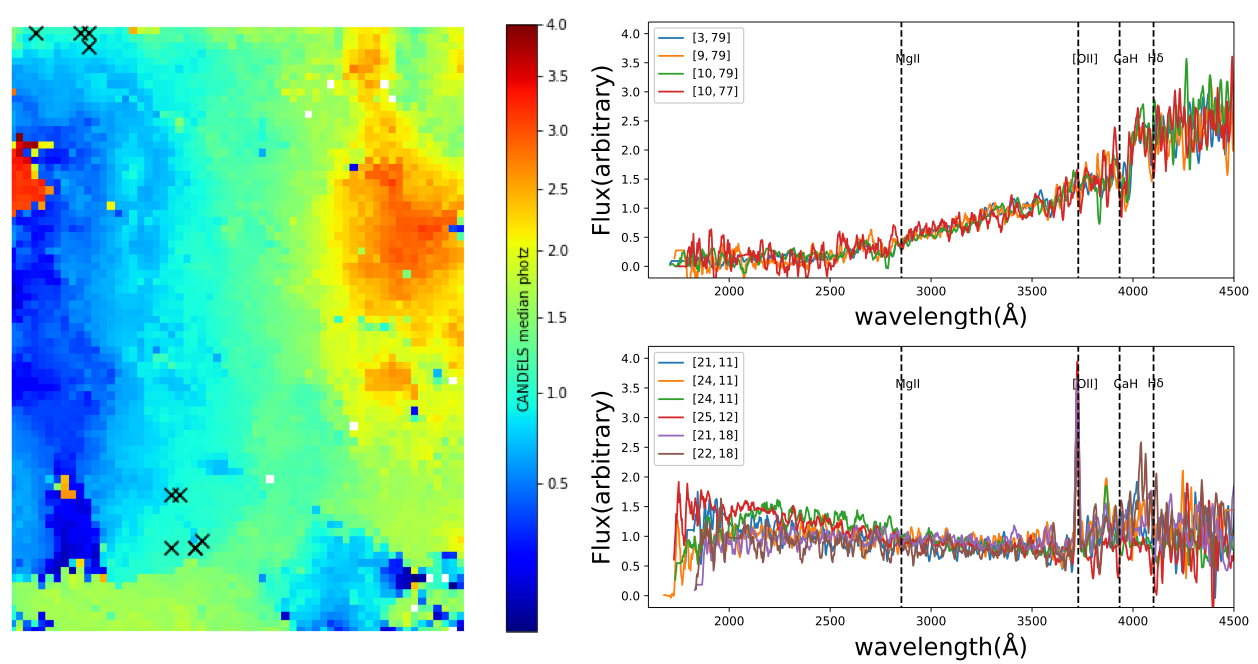
\includegraphics[width=0.55\textwidth]{figs/Hemmati18_Fig8_VVDS_spec.png}
\caption{\small {\it Left}: A Self-Organizing Map
\citep[SOM;][]{1990Natur.346...24K} from \citet{hemmati18} relating
LSST+WFIRST-like galaxy colors to redshift, $z$. FOBOS spectroscopic
training samples can be optimally designed to populate/calibrate
sparsely sampled regions. {\it Right}: Galaxy spectra from VVDS
\citep{2005A&A...439..845L} in SOM locations marked by black crosses.
More than just redshifts, the detailed similarity of spectral
features of galaxies localized within the SOM demonstrates
higher-level inferences (e.g. SFR) are possible given appropriate
training samples from FOBOS.} \label{fig:SOM} \end{wrapfigure}

\subsubsection{Cosmology with LBG--CMB cross correlation.}
\label{sec:LBG}

High-S/N CMB maps from next-generation CMB observatories (e.g., Simons Observatory and CMB-S4) will provide a cosmic
``reference background'' for measurements of gravitational lensing induced by matter along the line of sight.  After
cross-correlating with Lyman Break Galaxy (LBG) samples, a relatively flat lensing ``kernel'' with power at $z = 2$--5
enables powerful constraints on the Inflation-sensitive matter power spectrum, Horizon-scale General Relativity, cosmic
curvature and neutrino masses, and early Dark Energy \citep{ferraro19}.  \citet{wilson19} explore these constraints in
detail and highlight the need for spectroscopic determination of accurate redshift distributions for the employed LBG
samples. FOBOS would address this need in two ways.  First, several deep-drilling fields targeting $\sim$1000 LBGs BX,
$u$, $g$, and $r$ drop-out candidates per pointing ($\sim$10,000 deg$^{-2}$) would establish the interloper rate and
intrinsic redshift distribution of LBG samples to sufficient precision (this program would likely overlap with the
photo-$z$ program described above).  Second, $\sim$200 LBGs per pointing (2000 deg$^{-2}$) could be included as a
background program when FOBOS observes other sources across the sky, eventually building a 50-100 deg$^2$ data set of
sparse high-$z$ spectroscopy for LBG dN/d$z$ calibration via clustering redshifts \citep[see][]{wilson19}.


% \subsection{Kinematic weak lensing.}
% \label{sec:kinematic_lensing}

% Kinematic weak lensing is a promising new technique that measures shear in projected velocity fields of source galaxies to infer the presence of mass along the line-of-sight.  While compared to traditional photometric lensing, kinematic lensing requires more expensive resolved spectroscopy, it also yields shear measurements with 10 times the S/N per source galaxy \citep{huff13}.  This is because the result of velocity field lensing is uniquely defined whereas photometric lensing depends on the (unknown) intrinsic shape and orientation of the galaxy.  The kinematic lensing observable can be expressed as the offset between the kinematic major axis position angle (PA) and the photometric PA.  Small, 7-fiber IFU bundles can measure kinematic PAs to $\sim$1 degree precision (DiGiorgio in prep.), motivating a FOBOS deployment of 250 such IFUs per field that could measure mass profiles of galaxy cluster halos, perform targeted galaxy-galaxy lensing experiments, or provide checks on cosmological photometric lensing results from surveys like LSST.  Further work on developing this science case is underway. 



